\tasknumber{2018}{18} Высота равнобедренного треугольника $ABC$, опущенная из вершины B на основание $AC$ равна $a$? угол A равен $\alpha$. Найдите площадь треугольника.
\begin{figure}[h]
\centering
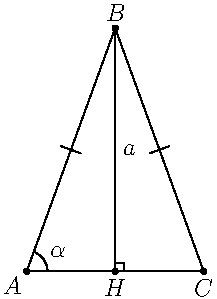
\includegraphics[scale =1.0]{pic18.pdf}
\end{figure}\\

\Solution
 В $\triangle ABH$: $\tg\angle A =\dfrac{BH}{AH}$. Следовательно: $AH=\dfrac{BH}{\tg\angle A}=\dfrac{a}{\tg\alpha}$
По свойству высоты в равнобедренном треугольнике, высота является медианой. Тогда:
\begin{center}$
AH=HC=\dfrac{a}{\tg\alpha}\rightarrow AC=AH+HC=\dfrac{2a}{\tg\alpha}
 $\end{center}
По формуле площади для треугольника получаем:
\begin{center}$
S(ABC)=\dfrac{1}{2}\cdot BH\cdot AC=\dfrac{1}{2}\cdot\dfrac{2a}{\tg\alpha}\cdot a=\dfrac{a^2}{\tg\alpha}=a^2\cdot\ctg\alpha
 $\end{center}
\Answer{$a^2\cdot\ctg\alpha$}


